\chapter{I test sulle prestazioni}

In questo capitolo verranno analizzati i test affrontati per valutare la reale bontà delle scelte fin qui discusse per quanto riguardo le due funzioni critiche di un filesystem: la \emph{read} e la \emph{write}.

Il motivo per chui si è scelto di analizzare solamente queste due funzioni è il seguente: sebbene l'intero filesystem dovrebbe essere ottimizzato, per la maggior parte del codice non è stato possibile implementare strategie alternative a quelle realizzate dal momento che il vero \emph{bootlneck} è il database, ed anche diminuendo il numero di istruzioni scritte non sarebbe diminuita la complessità generale del sistema.

Come abbiamo visto invece nel capitolo precedente, nel realizzare la persistenza di dati binari si è reso necessario compiere delle scelte che, come vedremo, comportano significative differenze.

\section{L'analisi della persistenza dei dati}
In questo paragrafo verranno presentate le possibili scelte realizzative che si sono prese in considerazione nell'implenetazione della persistenza dei dati binari.

In tutto il progetto il requisito fondamentale che è stato sempre rispettato è stata la flessibilità, intesa a tutto tondo: possibilità di sostituire il backend, possibilità di scalare orizzontalmente su un cluster di macchine e non porre limiti a quello che un utente, o un gruppo di essi, può fare con il suo filesystem, coerentemente con una gestione dei permessi di tipo Unix-like.

Proprio quest'ultimo aspetto della modularità è stato affrontato nella realizzazione delle due funzioni che trattano dati binari; non si è voluto stabilire un limite massimo per la dimensione dei file memorizzati nel database (se non quello imposto dal dispositivo fisico su cui si lavora).

Prima di giungere a come il problema è stato risolto è opportuno ricordare come un filesystem comune funziona: almeno per quanto ci possa interessare, è possibile distinguere inode e blocchi di dati; nei primi sono memorizzati i metadati ed i puntatori ai secondi\footnote{Questa è un'approssimazione, in quanto un inode contiene un blocco di puntatori a dati, e due puntatori a blocchi di altri puntatori a dati}. 

La prima soluzione ideata prevedeva che un solo array di byte si occupasse di memorizzare l'intero file binario; si può ben capire che questa tecnica può essere sufficiente fin quando un file è di piccole dimensioni, ma non è più sufficiente per la gestione di grandi quantità di dati, in quanto la lettura, fosse anche di un solo byte, avrebbe richiesto il caricamento in memoria dell'intero array, e poichè lo spazio nello \emph{heap} della Virtual Machine è limitato questa soluzione è apparsa da subito improponibile. Per di più, nel caso di un ridimensionamento del file si sarebbe reso necessario copiare in un nuovo array tutti i dati da salvare, operazione banale da un punto di vista algoritmico, ma decisamente complessa meno da un punto di vista computazionale e di memoria (lo spazio necessario sarebbe diventato la somma di quello necessario per contenere entrambi).

Una seconda soluzione, nata dalla precedente, prevedeva, invece di un solo array di byte, un array di array di byte, che sarebbero stati tutti dimensionati a 0, ed allocati al momento del bisogno. Questa soluzione è stata immediatamente abbandonata perchè sofferente di un problema ancor maggiore della precedente: gli array di byte avrebbero rappresentato i dati salvati, ma poichè l'array di array è inizializzato ad una dimensione fissa, sarebbe stato necessario imporre all'utente dei vincoli sulla dimensione massima dei file memorizzati (se ad esempio abbiamo blocchi da 512kB e fosse stato allocato in memoria un array di array di dimensione 50, la dimensione massima sarebbe stata 25600kB).

A questo punto è stato deciso di sacrificare, parzialmente, le performance globali sostituendo l'array di array con un ArrayList, che garantisce le stesse funzionalità della soluzione precedente, senza però imporre un vincolo sulla dimensione massima.

Infine, analizzando la documentazione di OrientDB, è stato possibile trovare una quarta possibilità, propria del database, utilizzando il record ORecordBytes, appositamente studiato per dati binari, in sostutuzione dell'array di byte e mantenendo l'ArrayList.

Nel corso del prossimo capitolo verranno analizzati i risultati dei test che hanno confrontato la terza e la quarta soluzione, spiegando poi perchè la scelta sia ricaduta su quest'ultima.

\subsection{Come sono stati condotti i test}
Prima di presentare i risultati dei test è necessario dedicare qualche parola per descrivere come i test sono stati condotti.

Innanzi tutto per confrontare le due versioni è stato necessario creare due versioni della classe che implementa la read e la write, ciascuna delle quali realizza una soluzione diversa, e quindi sono stati ottenuti due pacchetti \emph{jar} differenti. Poichè il progetto presentato è una libreria, è stato realizzato un metodo \emph{main}, in modo da rendere il pacchetto eseguibile, che esegue azioni diverse in base ai parametri con cui viene lanciato.

Oltre a ciò è stato scritto un semplice script bash in modo da rendere automatica l'esecuzione dei test, ciascuno dei quali è stato ripetuto con una dimensione dei blocchi di allocazione man mano crescente per dieci volte, così da ridurre al minimo la possibilità che il risultato sia legato al carico complessivo del sistema operativo.

Il test è stato così condotto: da un file binario la cui dimensione è 26.1MB viene estratta la sua sequenza di byte che è poi memorizzata in un array di byte. Poi, a seconda che sia richiesta una lettura, una scrittura o entrambe, il sistema si comporta di conseguenza. L'istruzione precedente, così come la successiva, all'invocazione del metodo richiesto è una chiamata della funzione \emph{System.currentTimeMillis()}, ed il tempo di esecuzione viene calcolato effettuando una sottrazione tra i due tempi: il risultato così ottenuto è preciso al millesimo di secondo.

\section{Il test di scrittura}
In questo paragrafo saranno analizzati i risultati dei test condotti sull'operazione di scrittura di dati. Come abbiamo detto il numero di byte memorizzati è 26$^{.}$056$^{.}$704, e non sono stati generati in maniera casuale dal sistema, ma sono byte estratti da un file concreto.

I risultati, va sottolineato, forniscono un \emph{upper bound} sul tempo effettivamente richiesto, dal momento che, al termine di ogni esecuzione, il database è stato cancellato per costringere il sistema a creare nuovi record senza permettere il riciclo di quelli vecchi; come abbiamo visto, infatti, nuovi blocchi vengono allocati dinamicamente solo se necessario in quanto questa è un'operazione computazionalmente pesante e che richiede molto tempo\footnote{Ad esempio, l'operazione di sovrascrittura non prevede alcuna allocazione di nuovi record}. Si garantisce quindi che, a regime, il tempo necessario per la scrittura effettivamente necessario sarà \emph{mediamente} minore.

Nelle figure 5.1 e 5.2 sono riportati i risultati dei test, che sono abbastanza significativi.

\begin{figure}
\centering
\begin{tabular}{cccccccc}
\toprule
\textbf{} & \textbf{1kB} & \textbf{2kB} & \textbf{4kB} & \textbf{16kB} & \textbf{64kB} & \textbf{256kB} & \textbf{1MB}\\
\midrule
ORecordBytes & 3266.8 & 2356.4 & 1506.8 & 691.3 & 322.2 & 170.7 & 122.8 \\
Array di byte & 1139.7 & 1058.9 & 1053.5 & 1019.9 & 1060.6 & 1049.7 & 1066.8\\
Differenza & 2127.1 & 1297.5 & 453.3 & -328.6 & -738.4 & -879.0 & -944\\
\bottomrule
\end{tabular}
\caption{Tabella che elenca i tempi medi di scrittura (espressi in ms) nelle due soluzioni in base alle dimensioni dei blocchi allocati e loro differenza}
\label{:}
\end{figure}

\begin{figure}
\centering
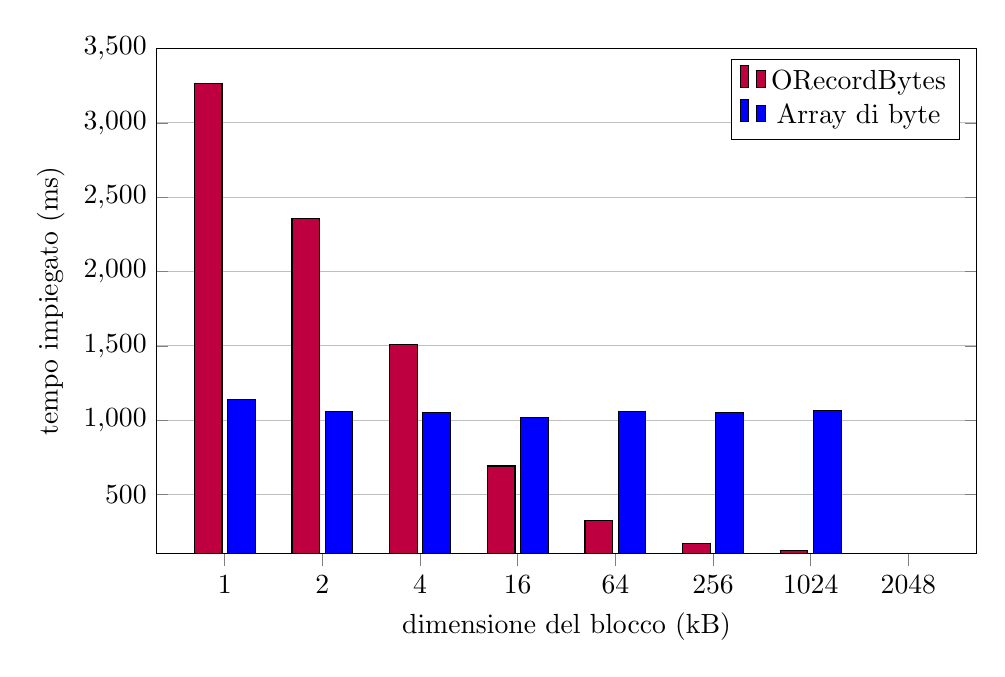
\begin{tikzpicture}
\begin{axis} [ylabel={tempo impiegato (ms)}, xlabel={dimensione del blocco (kB)},
ybar,ymin=100,ymax=3500,xtick=data,
ymajorgrids=true,xtick pos=left,
symbolic x coords={$1$,$2$,$4$,$16$,$64$,$256$,$1024$, $2048$},
title style={align=center}, width=12cm, height=8cm]
\addplot
[fill=purple,
draw=black] coordinates
{($1$, 3266.8) ($2$, 2356.4)
($4$, 1506.8) ($16$, 691.3)
($64$, 322.2) ($256$, 170.7)
($1024$, 122.8) ($2048$, 5)};
\addplot
[fill=blue,
draw=black] coordinates
{($1$, 1139.7) ($2$, 1058.9)
($4$, 1053.5) ($16$, 1019.9)
($64$, 1060.6) ($256$, 1049.7)
($1024$, 1066.8) ($2048$, 5)};
\legend{ORecordBytes,Array di byte}
\end{axis}
\label{1}
\end{tikzpicture}
\caption{Grafico del tempo impiegato per la memorizzazione di un file da 26,1MB}
\label{:}
\end{figure}

Come è possibile apprezzare, l'implementazione degli ORecordBytes permette una sensibile variazione delle performance al variare della dimensione dei blocchi allocati (principalmente a causa del fatto che la creazione di oggetti di tipo ORecordBytes è molto più costosa della semplice allocazione in memoria di un array di byte). Questa differenza, però, svanisce non appena diminuisce il numero di record allocati: infatti, mentre la soluzione che prevede gli array di byte mantiene (quasi) costante il suo tempo di esecuzione, l'altra soluzione, nel passare da un blocco di dimensione 1kB ad uno di dimensione 1MB, lo abbatte di un fattore 26, passando da 3266.8ms a 122.8ms.

Naturalmente aumentare la dimensione dei blocchi è un'operazione non priva di costi aggiuntivi visto che allocare spazio extra significa generare sprechi. Statisticamente, lo spazio eccedente occupato ma non sfruttato è la metà della dimensione del blocco. Va quindi ben ponderata la scelta di quanto spazio dedicare a cisacun record, considerando anche che, ad oggi, non è previsto di poterlo modificare.

Una possibile spiegazione al motivo per cui la soluzione che prevede l'array di byte non è sensibile alla variazione della dimensione dei blocchi (i tempi di esecuzione differiscono al massimo di 120ms, e raggiungono il loro minimo con dimensione 16kB) è che il sistema non prevede tuning specifici; inoltre questa soluzione prevede sempre e comunque che un file venga caricato interamente nello heap per poterlo manipolare, con conseguente appesantimento del sistema.

\section{Il test di lettura}
Successivamente sono stati eseguiti i test di lettura del file appena scritto. Va evidenziato che per non sfruttare potenzialità proprie di OrientDB alla scrittura iniziale e ad ogni lettura è stata fatta seguire una chiusura del database, così da permettere un confronto equo tra le due soluzioni. La lettura richiesta è stata di tipo completo, ossia a partire dalla posizione 0 per tutto il file. Questo non comporta falsificazioni del risultato finale visto che, in entrambe le implementazioni, posizionarsi in una posizione qualsiasi del file introduce un overhead nullo.

\begin{figure}[t]
\centering
\begin{tabular}{cccccccc}
\toprule
\textbf{} & \textbf{1kB} & \textbf{2kB} & \textbf{4kB} & \textbf{16kB} & \textbf{64kB} & \textbf{256kB} & \textbf{1MB}\\
\midrule
ORecordBytes & 3764.5 & 1782.4 & 1062.2 & 462.4 & 237.4 & 127.3 & 134.9 \\
Array di byte & 2873.0 & 2816.9 & 2853.1 & 2778.4 & 2842.5 & 2866.3 & 2867.7\\
Differenza & 891.5 & -1034.5 & -1790.9 & -2316.0 & -2605.1 & -2739.0 & -2732.8\\
\bottomrule
\end{tabular}
\caption{Tabella che elenca i tempi medi di lettura (espressi in ms) nelle due soluzioni in base alle dimensioni dei blocchi allocati e loro differenza}
\label{:}
\end{figure}
\begin{figure}
\centering
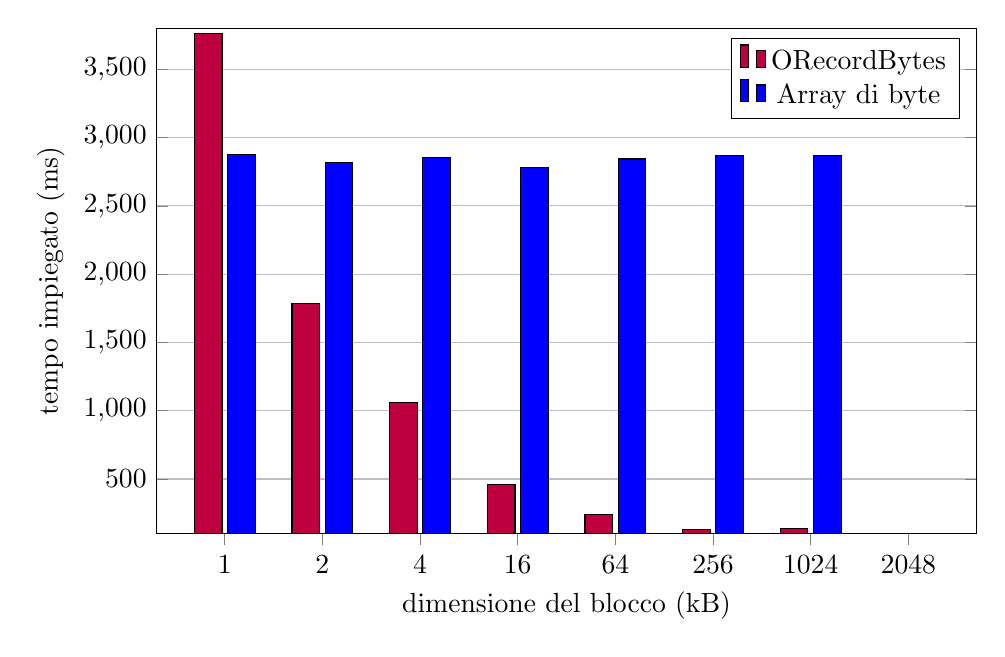
\begin{tikzpicture}
\begin{axis} [ylabel={tempo impiegato (ms)}, xlabel={dimensione del blocco (kB)},
ybar,ymin=100,ymax=3800,xtick=data,
ymajorgrids=true,xtick pos=left,
symbolic x coords={$1$,$2$,$4$,$16$,$64$,$256$,$1024$, $2048$},
title style={align=center}, width=12cm, height=8cm]
\addplot
[fill=purple,
draw=black] coordinates
{($1$, 3764.5) ($2$, 1782.4)
($4$, 1062.2) ($16$, 462.4)
($64$, 237.4) ($256$, 127.3)
($1024$, 134.9) ($2048$, 5)};
\addplot
[fill=blue,
draw=black] coordinates
{($1$, 2873) ($2$, 2816.9)
($4$, 2853.1) ($16$, 2778.4)
($64$, 2842.5) ($256$, 2866.3)
($1024$, 2867.7) ($2048$, 5)};
\legend{ORecordBytes,Array di byte}
\end{axis}
\label{1}
\end{tikzpicture}
\caption{Grafico del tempo impiegato per la lettura di un file da 26,1MB}
\label{:}
\end{figure}

Anche in questo caso, come riportato nelle figure 5.3 e 5.4, si confermano i dati ottenuti nel test precedente, ossia l'uso di ORecordBytes permette una diminuzione massima dei tempi di esecuzione pari a 2732.8ms rispetto alla soluzione che fa uso degli array di byte.

Va notato che però, a differenza dei risultati ottenuti in lettura, la diminuzione dei tempi di esecuzione non è costante, ma, nel passaggio della dimensione dei blocchi da 256kB ad 1MB risulta essere di segno opposto.

Un'ultima annotazione riguarda un confronto tra i tempi di lettura e quelli di scrittura è la seguente: generalmente i tempi di lettura di un dispositivo, a parità di dimensione richiesta, sono minori, ma in questo caso accade il contrario. Questo è indice di cosa in realtà accade in ORecordBytes: quando si chiede a quest'oggetto di memorizzare, in realtà viene semplicemente copiato un array già presente in memoria, mentre quando viene richiesto di trasformare il suo contenuto in un array di byte il sistema deve allocare dello spazio aggiuntivo non previsto nello heap.

\subsection{OrientDB e la cache}
Nel test precedente per evitare di sfruttare tutte le peculiarità di ORecordBytes non disponibili per le altre soluzioni si è agito evitando di utilizzare la cache. Anche in questo caso, quindi, si è trovato un upper bound (affermazione falsa per quanto riguarda la soluzione che prevede gli array di byte).

Volendo vedere qual è la prestazione massima effettivamente fruibile in lettura è stato fatto un test così strutturato: un file viene scritto, poi, senza chiudere il database, ne viene richiesta la lettura. 

\begin{figure}
\centering
\begin{tabular}{cccccccc}
\toprule
\textbf{} & \textbf{1kB} & \textbf{2kB} & \textbf{4kB} & \textbf{16kB} & \textbf{64kB} & \textbf{256kB} & \textbf{1MB}\\
\midrule
Con cache & 2334.1 & 1432.7 & 406.7 & 144.2 & 43.6 & 27.0 & 22.7\\
Senza cache & 3764.5 & 1782.4 & 1062.2 & 462.4 & 237.4 & 127.3 & 134.9 \\
Differenza & -1430.4 & -349.7 & -655.5 & -318.2 & -139.8 & -100.3 & -112.2\\
\bottomrule
\end{tabular}
\caption{Tabella che elenca i tempi medi di lettura (espressi in ms) nelle due soluzioni in base alle dimensioni dei blocchi allocati e loro differenza}
\label{:}
\end{figure}

\begin{figure}
\centering
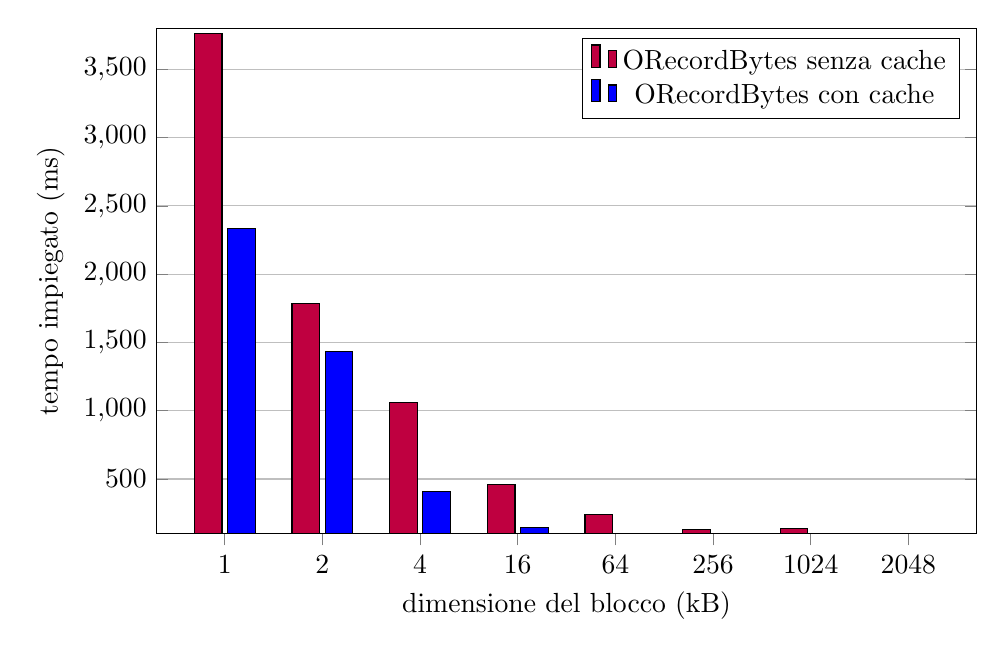
\begin{tikzpicture}
\begin{axis} [ylabel={tempo impiegato (ms)}, xlabel={dimensione del blocco (kB)},
ybar,ymin=100,ymax=3800,xtick=data,
ymajorgrids=true,xtick pos=left,
symbolic x coords={$1$,$2$,$4$,$16$,$64$,$256$,$1024$, $2048$},
title style={align=center}, width=12cm, height=8cm]
\addplot
[fill=purple,
draw=black] coordinates
{($1$, 3764.5) ($2$, 1782.4)
($4$, 1062.2) ($16$, 462.4)
($64$, 237.4) ($256$, 127.3)
($1024$, 134.9) ($2048$, 5)};
\addplot
[fill=blue,
draw=black] coordinates
{($1$, 2334.1) ($2$, 1432.7)
($4$, 406.7) ($16$, 144.2)
($64$, 43.6) ($256$, 27)
($1024$, 22.7) ($2048$, 5)};
\legend{ORecordBytes senza cache,ORecordBytes con cache}
\end{axis}
\label{1}
\end{tikzpicture}
\caption{Grafico del tempo impiegato per la lettura di un file da 26,1MB senza e con cache}
\label{:}
\end{figure}

Il risultato è riportato nelle figure 5.5 e 5.6, ed è sintetizzabile facendo notare come usare la cache significa ottenere un risparmio medio del 61,68\%, con punte minime di 19,62\% e punte massime di 83,17\%. Questo perchè i record non vengono effettivamente caricariti e riscaricati sul disco, ma rimangono in memoria e vengono automaticamente recuperati dall'engine del database quando sono richiesti. In quest'ottica è anche spiegabile come mai il risparmio di tempo è crescente: il numero di record da leggere è inversamente proporzionale alla dimensione del blocco usato, quindi, minori sono i record utilizzati e minore sarà il numero di letture effettivamente da disco da effettuare (infatti il numero totale di record mantenibili in cache è pressochè costante).